%% LyX 2.4.4 created this file.  For more info, see https://www.lyx.org/.
%% Do not edit unless you really know what you are doing.
\documentclass[english]{article}
\usepackage[T1]{fontenc}
\usepackage[latin9]{inputenc}
\usepackage{units}
\usepackage{enumitem}
\usepackage{amsmath}
\usepackage{amsthm}
\usepackage{geometry}
\geometry{verbose,tmargin=1in,bmargin=1in,lmargin=1in,rmargin=1in}

\makeatletter
%%%%%%%%%%%%%%%%%%%%%%%%%%%%%% Textclass specific LaTeX commands.
\numberwithin{equation}{section}
\numberwithin{figure}{section}
\newlength{\lyxlabelwidth}      % auxiliary length 

%%%%%%%%%%%%%%%%%%%%%%%%%%%%%% User specified LaTeX commands.
\usepackage{fancyhdr}
\usepackage{lastpage}
\pagestyle{fancy}
\usepackage{enumitem}
\usepackage{ifthen}
\everymath=\expandafter{\the\everymath\displaystyle}
%\DeclareMathSizes{10}{10}{10}{10}
\usepackage{multicol}

\usepackage{tikz}
\usepackage{tikz-3dplot}
\usetikzlibrary{calc,arrows}

\usetikzlibrary{patterns}
\usetikzlibrary{plotmarks}
\usepackage{pgfplots}
\pgfplotsset{compat=newest}
\usepgfplotslibrary{polar}

\usepackage{calc}
\usepackage[nomessages]{fp}

\usepackage{datetime}
% Added by lyx2lyx
\setlength{\parskip}{\smallskipamount}
\setlength{\parindent}{0pt}

\makeatother

\usepackage{babel}
\begin{document}
\renewcommand{\author}{Dr.\,James Ashe}

\newcommand{\classNum}{331}

\newcommand{\classSec}{A}

\newcommand{\examType}{Exam 2}

\newcommand{\nameType}{Solutions}

\renewcommand{\date}{\formatdate{7}{10}{2013}}

%%First page's header%%%%%%%%%%%%%%%%%%%%%%
\fancypagestyle{firststyle} %%header settings for first pagr
{
	\fancyhead[L]{MTH \classNum{}(\classSec{}) \author{}\\
	\textbf{\examType{}} ~\date{}}
	\fancyhead[C]{\textbf{\nameType}}
	%\fancyhead[R]{\textbf{Name:\hspace{5cm}}}
	\setlength{\headsep}{14pt}
}
%%%%%%%%%%%%%%%%%%%%%%%%%%%%%%%%%%%%%%%%%%

%%Next page's header%%%%%%%%%%%%%%%%%%%%%%%
\setlist{nolistsep}
\lhead{MTH \classNum{}(\classSec{})} 
\chead{\textbf{\nameType}} 
\cfoot{\thepage{}~of~\pageref{LastPage}} 
\setlength{\headsep}{5pt} 
%%%%%%%%%%%%%%%%%%%%%%%%%%%%%%%%%%%%%%%%%%%

%%Various settings; see the preamble for other settings%%%%%
%\setenumerate[0]{leftmargin=12pt,itemindent=0pt,labelwidth=0pt}
\setlist{topsep=.5pt}
\renewcommand{\labelenumi}{\textbf{\arabic{enumi}.}}
\renewcommand{\labelenumii}{\textbf{\alph{enumii}.}}
\thispagestyle{firststyle}
%%%%%%%%%%%%%%%%%%%%%%%%%%%%%%%%%%%%%%%%%%

\newcommand{\xmax}{0}
\newcommand{\xmin}{-\xmax}
\newcommand{\xstep}{0}
\newcommand{\ymax}{0}
\newcommand{\ymin}{-\ymax}
\newcommand{\ystep}{0} 
\newcommand{\dspace}{\vspace{1cm}}
\newcommand{\xa}{0}
\newcommand{\xb}{0}
\newcommand{\ya}{1}
\newcommand{\yb}{1}

\newcommand{\xspace}{\vspace{1cm}}

\textbf{Justify your answers and show your work. Unless stated otherwise,
all questions worth 5pts.}

\emph{Determine the radius of convergence of the following power series.
Then test the endpoints to determine the interval of convergence.}
\begin{enumerate}[resume]
\item ${\displaystyle \sum\left(\frac{x}{3}\right)^{k}}$

\begin{enumerate}[resume]
\item []Using the root test, ${\displaystyle \lim_{n\rightarrow\infty}}\sqrt[n]{\left|\left(\frac{x}{3}\right)^{n}\right|}={\displaystyle \lim_{n\rightarrow\infty}}\left|\frac{x}{3}\right|=\left|\frac{x}{3}\right|<1$
when $-3<x<3$. So the radius of convergence is$\left(-3,3\right)$.\\
For the endpoints, $x=-3\Rightarrow\sum\left(-1\right)^{k}$ diverges,
and $x=3\Rightarrow\sum1$ diverges. So then the interval of convergence
is $(-3,3)$.
\item []Alternatively note that $\sum\left(\frac{x}{3}\right)^{k}$ is
a geometric series with ratio $\frac{x}{3}$. So it converges when
$3<x<-3$.\vfill
\end{enumerate}
\item ${\displaystyle \sum\left(-1\right)^{k}\frac{x^{k}}{5^{k}}}$

\begin{enumerate}[resume]
\item []Using the root test, ${\displaystyle \lim_{n\rightarrow\infty}}\sqrt[n]{\left|\left(\frac{-x}{5}\right)^{n}\right|}={\displaystyle \lim_{n\rightarrow\infty}}\left|-\frac{x}{5}\right|=\left|-\frac{x}{5}\right|<1$
when $-5<x<5$. So the radius of convergence is$\left(-5,5\right)$.\\
For the endpoints, $x=-5\Rightarrow\sum\left(-1\right)^{k}\frac{(-5)^{k}}{5^{k}}=\sum\frac{(5)^{k}}{5^{k}}=\sum1$
diverges, and $x=5\Rightarrow\sum\left(-1\right)^{k}\frac{5^{k}}{5^{k}}=\sum\left(-1\right)^{k}$
diverges. So then the interval of convergence is $(-5,5)$.
\item []Alternatively note that ${\displaystyle \sum\left(-1\right)^{k}\frac{x^{k}}{5^{k}}}=\sum\left(-\frac{x}{5}\right)^{k}$
is a geometric series with ratio $-\frac{x}{5}$. So it converges
when $-5<x<5$.\vfill
\end{enumerate}
\end{enumerate}
\emph{Use the geometric series ${\displaystyle \sum_{k=0}^{\infty}x^{k}=\frac{1}{1-x}}$,
for $\left|x\right|<1$ to find a power series representations for
the following functions, and determine the interval of convergence.}
\begin{enumerate}[resume]
\item $f(3x)=\frac{2}{1-3x}$.

\begin{enumerate}[resume]
\item []Let $a=2$ and $r=3x$. So then $\frac{2}{1-3x}={\displaystyle \sum_{k=0}^{\infty}2(3x)^{k}}$
when $\left|3x\right|<1$. The interval of convergence is $\left(-\nicefrac{1}{3},\nicefrac{1}{3}\right)$.\vfill
\end{enumerate}
\end{enumerate}
\emph{Express the following }\textbf{\emph{polar}}\emph{ coordinates
in }\textbf{\emph{Cartesian}}\emph{ coordinates.}
\begin{enumerate}[resume]
\item $\left(4,5\pi\right)$

\begin{enumerate}[resume]
\item []$x=4\cos(5\pi)=-4$ and $y=4\sin(5\pi)=0$. So,\\
$(-4,0)$.\vfill
\end{enumerate}
\end{enumerate}
\emph{Express the following }\textbf{\emph{Cartesian}}\emph{ coordinates
in }\textbf{\emph{polar}}\emph{ coordinates in at least }\textbf{\emph{two}}\emph{
different ways. }
\begin{enumerate}[resume]
\item $\left(-1,\sqrt{3}\right)$

\begin{enumerate}[resume]
\item []$r^{2}=(-1)^{2}+(\sqrt{3})^{2}=4\Rightarrow r=2$\\
$\theta=\tan^{-1}\left(\frac{\sqrt{3}}{-1}\right)=-\frac{\pi}{3}+\pi=\frac{2\pi}{3}$
(add $\pi$ since the point is in quadrant II). So, \\
$(2,\frac{2}{3}\pi)$.\vfill
\end{enumerate}
\end{enumerate}
\newpage

\emph{Use the parametric curve $x=t^{2}+1$ and $y=1-t$ for $-\infty<t<\infty$
to complete problems \ref{enu:Plot-the-parametric}-\ref{enu:Find-the-slope}. }
\begin{enumerate}[resume]
\item \label{enu:Plot-the-parametric}Sketch the parametric curve.

\begin{enumerate}[resume]
\item []\renewcommand{\xmax}{10}
\renewcommand{\xmin}{-1}
\renewcommand{\xstep}{0} %must be xmin+n
\renewcommand{\ymax}{10}
\renewcommand{\ymin}{-10}
\renewcommand{\ystep}{0} %must be ymin+n
%%%%%%%
\begin{tikzpicture} 
\begin{axis}[height=5cm, 
	width=5cm, 
	axis lines=middle,
	%minor x tick num={4},
	%minor y tick num={4},
	%grid=both,
	ticks=none,
	%xtick={0,50,...,250},
	%ytick={0,10,20,...,40},
	%axis line style={-latex}, 
	xmin=\xmin,xmax=\xmax, 
	ymin=\ymin,ymax=\ymax,
	%restrict y to domain=-1:10,
	%no markers, 
	xlabel={$x$},ylabel={$y$}, 
	%every axis x label/.append style={anchor=north}, 
	%every axis y label/.append style={anchor=east}
	]
	
	%\addplot[color=black,solid,mark=*] coordinates {(0,1)} node[right] {\footnotesize{$(0,1)$}};

	\addplot[domain=-3:3,thick,samples=100,draw=red,<->] (x*x+1,1-x) node[pos=.525,right] {$$};
	
\end{axis}
\end{tikzpicture}\vfill
\end{enumerate}
\item Eliminate the parameter to obtain an equation in $x$ and $y$.

\begin{enumerate}[resume]
\item []$y=1-t\Rightarrow t=1-y\Rightarrow x=(1-y)^{2}+1$.\vfill
\end{enumerate}
\item Find the slope of the tangent line when $t=4$.

\begin{enumerate}[resume]
\item []$\frac{dy}{dx}=\frac{\nicefrac{dy}{dt}}{\nicefrac{dx}{dt}}=\frac{-1}{2t}$.
So when $t=4$ the tangent line has slope, $-\frac{1}{8}$.\vfill
\end{enumerate}
\item \label{enu:Find-the-slope}Find when the tangent line to the curve
is a vertical line. 

\begin{enumerate}[resume]
\item []$\frac{dy}{dx}=\frac{\nicefrac{dy}{dt}}{\nicefrac{dx}{dt}}=-\frac{1}{2t}$
is undefined when $2t=0\Rightarrow t=0$.\vfill
\end{enumerate}
\end{enumerate}
\emph{Locate the following polar coordinates on the graph. }
\begin{enumerate}[resume]
\item A:$\left(1.5,\frac{\pi}{6}\right)$, B:$\left(-1.5,\frac{\pi}{6}\right)$,
C:$\left(1.5,\frac{\pi}{6}+3\pi\right)$, D:$\left(1.5,\frac{\pi}{6}-8\pi\right)$

\begin{enumerate}[resume]
\item []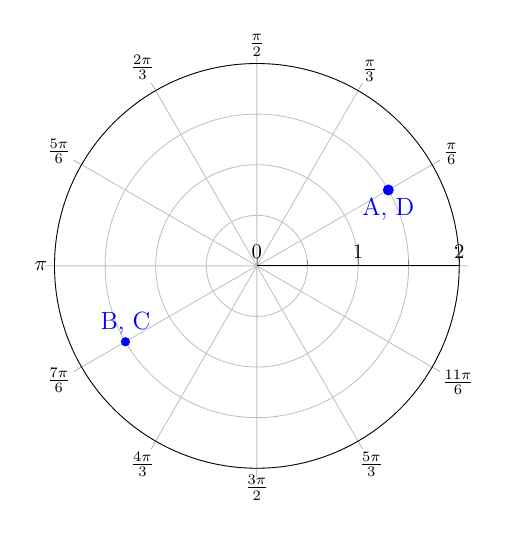
\begin{tikzpicture} [scale=.75] 
	\begin{polaraxis}[
			xmin=0,xmax=360,
			ymin=0,ymax=2,
			ytick={0,1,...,20}, 
			%minor x tick num={4},
			minor y tick num={1},
			grid=both,
			%yticklabels={,,,1,,,2,,}, 
			xticklabels={,,$\frac{\pi}{6}$,$\frac{\pi}{3}$,$\frac{\pi}{2}$,$\frac{2\pi}{3}$,$\frac{5\pi}{6}$,$\pi$,$\frac{7\pi}{6}$,$\frac{4\pi}{3}$,$\frac{3\pi}{2}$,$\frac{5\pi}{3}$,$\frac{11\pi}{6}$,}
		]
		%\addplot+[black, very thick, mark=none, domain=0:720, samples=600 ] {2-5*cos(x)};
		%\addplot+[gray, very thin, mark=none, domain=0:720, samples=600 ] {1.5};
		%\addplot+[black, mark = *, nodes near coords=mylabel,every node near coord/.style={anchor=180}] coordinates ( 30: 1.5);
		%\draw (30:1.5) circle[radius=2pt];
		\addplot[color=blue,solid,mark=*,very thick] coordinates {(30,1.5)} node[below] {\large{A, D}};
		\addplot[color=blue,solid,mark=*] coordinates {(30,-1.5)} node[above] {\large{B, C}};
		%\addplot[color=blue,solid,mark=*] coordinates {(120,1.5)} node[right] {\footnotesize{C}};
		%\addplot[color=blue,solid,mark=*] coordinates {(30,1.5)} node[right] {\footnotesize{D}};
	\end{polaraxis}
	%\draw (3.43cm,-.7cm) node [below] {$r=2-5\cos\theta $}; 
\end{tikzpicture}\vfill
\end{enumerate}
\end{enumerate}
\newpage

\emph{Use the polar equation $r=3-\cos\theta$ to complete problems
\ref{enu:Graph-the-polar}-\ref{enu:=00005B10-pts=00005D-Find}.}
\begin{enumerate}[resume]
\item \label{enu:Graph-the-polar}Graph the polar equation.

\begin{enumerate}[resume]
\item []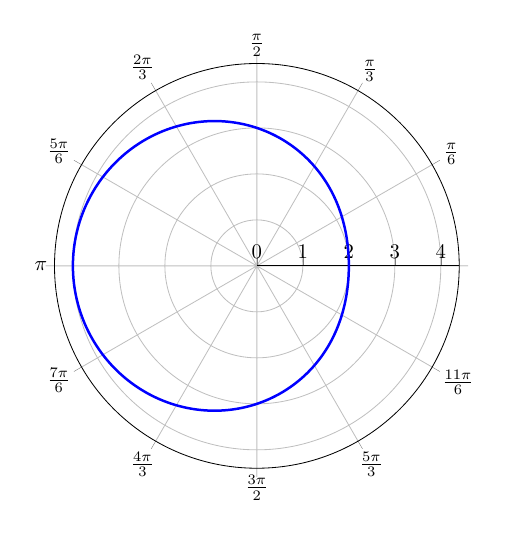
\begin{tikzpicture} [scale=.75] 
	\begin{polaraxis}[
			%xmin=0,xmax=360,
			%ymin=0,ymax=2,
			%ytick={0,1,...,20}, 
			%minor x tick num={4},
			%minor y tick num={1},
			grid=both,
			%yticklabels={,,,1,,,2,,}, 
			xticklabels={,,$\frac{\pi}{6}$,$\frac{\pi}{3}$,$\frac{\pi}{2}$,$\frac{2\pi}{3}$,$\frac{5\pi}{6}$,$\pi$,$\frac{7\pi}{6}$,$\frac{4\pi}{3}$,$\frac{3\pi}{2}$,$\frac{5\pi}{3}$,$\frac{11\pi}{6}$,}
		]
		\addplot+[blue, very thick, mark=none, domain=0:360, samples=600 ] {3-cos(x)};

		%\addplot[color=blue,solid,mark=*] coordinates {(30,1.5)} node[right] {\footnotesize{A, D}};
		%\addplot[color=blue,solid,mark=*] coordinates {(30,-1.5)} node[right] {\footnotesize{B, C}};
		%\addplot[color=blue,solid,mark=*] coordinates {(120,1.5)} node[right] {\footnotesize{C}};
		%\addplot[color=blue,solid,mark=*] coordinates {(30,1.5)} node[right] {\footnotesize{D}};
	\end{polaraxis}
	%\draw (3.43cm,-.7cm) node [below] {$r=2-5\cos\theta $}; 
\end{tikzpicture}\vfill
\end{enumerate}
\item {[}10 pts{]} Find the slope of the tangent line when $\theta=\frac{\pi}{2}$.

\begin{enumerate}[resume]
\item []$r'=\sin\theta$\\
$\frac{dy}{dx}=\frac{\sin\theta\sin\theta+\left(3-\cos\theta\right)\cos\theta}{\sin\theta\cos\theta-\left(3-\cos\theta\right)\sin\theta}$
at $\theta=\frac{\pi}{2}\Rightarrow\frac{1+0}{0-3}=-\frac{1}{3}$\vfill
\end{enumerate}
\item \label{enu:=00005B10-pts=00005D-Find}{[}10 pts{]} Find the area enclosed
by the curve.
\begin{eqnarray*}
{\displaystyle \frac{1}{2}\int_{0}^{2\pi}\left(3-\cos\theta\right)^{2}\,d\theta} & = & \frac{1}{2}\int_{0}^{2\pi}9-6\cos\theta+\cos^{2}\theta\,d\theta\\
 & = & \frac{1}{2}\int_{0}^{2\pi}9-6\cos\theta+\frac{1+\cos2\theta}{2}\,d\theta\\
 & = & \frac{1}{2}\left[9\theta-6\sin\theta+\frac{1}{2}\theta+\frac{\sin2\theta}{4}\right]\bigg\vert_{0}^{2\pi}\\
 & = & \frac{1}{2}\left[18\pi-0+\pi+0\right]-\frac{1}{2}\left[0\right]\\
 & = & \frac{19}{2}\pi
\end{eqnarray*}
\end{enumerate}
%\begin{tikzpicture}[scale=2] 
	%\draw[color=red,domain=0:6.28,samples=200,smooth] plot (canvas polar cs:angle=\x 		r,radius={5-5*sin(\x r)});    %r = angle en radian 
%\end{tikzpicture}
\end{document}
